\prob{
    Let A be the matrix
    $$\bordermatrix{
            &   1   &   2   &   3   &   4   &   5   &   6   \cr
            &   1   &   0   &   0   &   1   &   1   &   0   \cr
            &   0   &   1   &   0   &   1   &   0   &   1   \cr
            &   0   &   0   &   1   &   0   &   1   &   1   
    }$$

    For q in $\{2,3\}$, let $M_q[A]$ be the vector matroid of $A$ when $A$ is viewed over $GF(q)$,
    the field of $q$ elements. Show that:

    \begin{enumerate}
        \item[(i)] 
            The sets of circuits of $M_2[A]$ and $M_3[A]$ are different.
        \item[(ii)]
            $M_2[A]$ is graphic but $M_3[A]$ is not.
        \item[(iii)] 
            $M_2[A]$ is represntable over $GF(3)$, but $M_3[A]$ is not representable over $GF(2)$.
    \end{enumerate} 
}

\begin{proof}\label{t1:p1}
    \begin{enumerate}[label=(\roman*)]
        \item\label{t1:p1:i}
            \ref{itm:name}
            Lets look for the circuits over $GF(2)$. As $0$ and $1$ are the only scalars over $GF(2)$,
            we can only pay attention to sums of the vector columns and forget about full linear combinations.\pn
            
            There are no loops, the only way to get a loop is having a zero column and it is not the case.\pn
            
            There are no circuits of length two (or parallel columns), the only way to get them is having two 
            exactly equal columns and it is not the case.\pn
            
            Lets call the columns 1, 2, and 3 the ``simple columns'', and the columns 4, 5 and 6 the ``double columns''.\pn
            
            For any pair of the columns from the simple columns there is a column from the double columns 
            such that the sum is zero. Such column is the one you can get from adding the chosen pair. 
            That is, $\{1, 2, 4\}$, $\{1, 3, 5\}$, $\{2, 3, 6\}$ are three dependent sets.\pn
            
            If you try to add all the simple columns, you can't add up to zero.\pn
            
            If you add two of the the double columns, you get the third one, so $\{4, 5, 6\}$ is dependent.\pn
            
            These four sets are circuits given that there are no smaller dependent sets.\pn
            
            These four are all the circuits of size three. Lets think about the circuits of size four.\pn
            
            Again, if you add two of the double columns, you get the third one, and there are two simple columns that can
            add up this third one. So, $\{1, 2, 5, 6\}$, $\{1, 3, 4, 6\}$, $\{2, 3, 4, 5\}$ are dependent sets.
            And no one of the four already given circuits are contained in them, so these are circuits themselves.\pn
            
            At any time you choose the three simple columns, you will get no way to add up to zero just adding double columns.
            So, any set containing all of the simple columns will not be a circuit.\pn
            
            If you choose all the double columns, you have already chosen a circuit, so if you add any other vector,
            you will get a dependent set that is not a circuit.\pn
            
            So these seven are all the circuits of $M_2[A]$.\pn
            
            Now lets look for the circuits over $GF(3)$. Again and for the same reason, there are not loops or parallel columns.\pn
            
            If you choose two simple colums and you add them, you get one of the double columns, so if you add to them the
            negative of this double column, you get the zero vector. So $\{1, 2, 4\}$, $\{1, 3, 5\}$, $\{2, 3, 6\}$ are
            circuits.\pn
            
            $\{4, 5, 6\}$ is not dependent, you can check that the determinant of their submatrix is $2$ (or -2 if you switched
            something).\pn
            
            If you choose two doble columns and add to them a simple one, again the determinant is not zero (it is always 1 or -1).
            So $\{1, 2, 4\}$, $\{1, 3, 5\}$, $\{2, 3, 6\}$ are all the circuits of size three.\pn
            
            Now lets look for circuits of size four.\pn
            
            If you choose two double columns and add one to the negative of the second one, you can find two simple columns that 
            can make them add up the zero vector (using the correct signs), these two vectors are exactly the ones that add up to
            the double column that you didn't choose. So none of these selections contains the circuits of size three and therefore
            they are circuits. So this give us the circuits $\{1, 2, 5, 6\}, \{1, 3, 4, 6\}, \{2, 3, 4, 5\}$.\pn
            
            If choose all of the double columns, you can choose any of the simple one so the four of them add up the zero vector using
            an appropiate selection for the signs. So this give us the dependent sets $\{1, 4, 5, 6\}, \{2, 4, 5, 6\}, \{3, 4, 5, 6\}$ 
            and they are circuits because any of the smaller circuits contain at least two simple columns.\pn
            
            The only other chance is choosing all of the simple columns, but wathever you add, you will get any of the three sized
            circuits as a subset. So these six are all of the circuits of size four.\pn
            
            There are no circuits of size five, because there are only two posibilities, having three simple columns and two double columns, 
            or having three double  columns and two simple columns. The first one, again contains as a subset a circuit of size three.
            The second one always contains as a subset a circuit of size four.\pn
            
            So in total, there are nine circuits for $M_3[A]$.\pn
                        
            Only by their cardinality, you can tell that the set of circuits of $M_2[A]$ and $M_3[A]$ are different.
            
        \item\label{t1:p1:ii}
            We are going to give a graphic representation of a graph that has $M_2[A]$ as an isomorphic matroid. You can
            verify that it has all the seven circuits that we gave previously and only those.\pn
            \begin{center}
                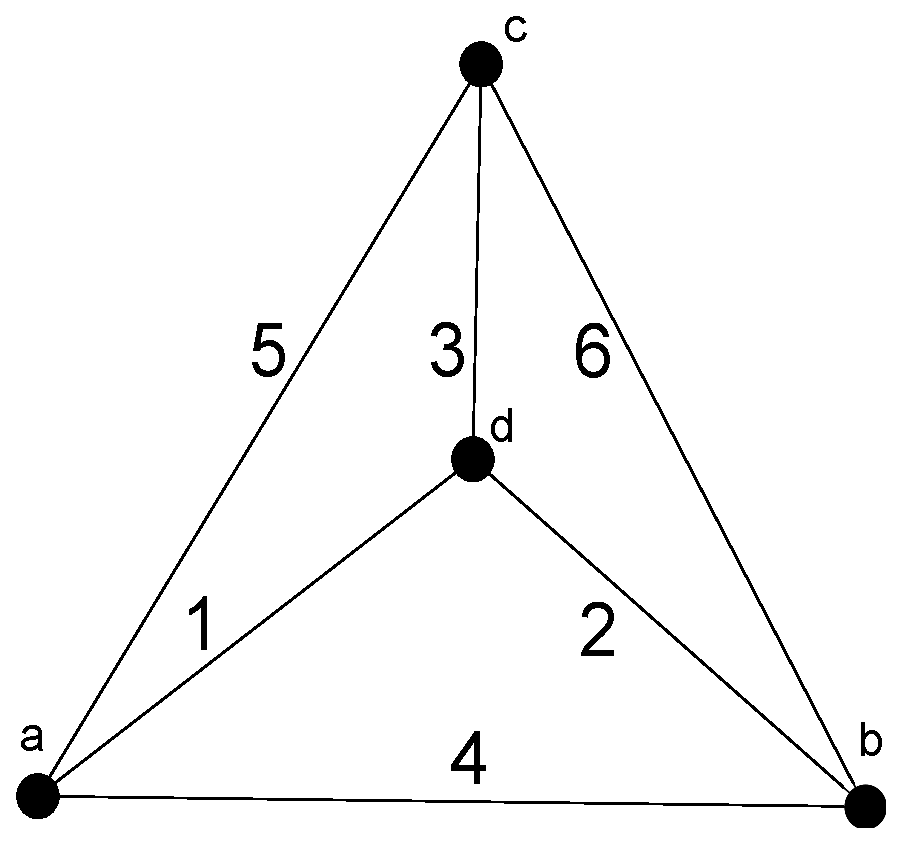
\includegraphics[width=7cm]{Test1/Problem1/tetrahedron.eps}
            \end{center}
            
            Now lets think what could happen if $M_3[A]$. For $M_3[A]$, we have the circuits 
            $\{1, 4, 5, 6\}, \{2, 4, 5, 6\}, \{3, 4, 5, 6\}$. Take any two of them, lets say
            $\{1, 4, 5, 6\}, \{2, 4, 5, 6\}$, they have three edges in common $\{4,5,6\}$. \pn
            
            If there is a graphic mathroid isomorphic to $M_3[A]$, $\{4,5,6\}$ defines three edges of a 
            $4$-cycle, that is, a $3$-trajectory. In any $3$-trajectory we will find $4$ vertices, so the fourth 
            edge is already determined by two of those vertices (the start vertex and the last vertex), but in this case 
            we have that $\{1, 4, 5, 6\}$, $\{2, 4, 5, 6\}$ are both $4$-cycles over the same set of vertices, 
            and so $1$ and $2$ have exactly the same two vertices, that is, they are parallel. But in [\ref{t1:p1}.\ref{t1:p1:i}]
            we saw that $M_3[A]$ has no parallel columns. So this is a contradiction.
        \end{enumerate}
\end{proof}